\documentclass[a4paper,10pt, spanish]{article}

\usepackage{graphicx}
\usepackage{listings}
\usepackage[final]{pdfpages}
\usepackage[spanish]{babel}
\usepackage[utf8]{inputenc}
\usepackage[export]{adjustbox}
\usepackage{mips}

\lstset{
language=C,
tabsize=2,
  basicstyle=\ttfamily,
  columns=fullflexible,
  frame=single,
  breaklines=true
}

\title{
            \large{Organización de Computadoras} \\
            \textbf{Trabajo Práctico 0} \\
            \textbf{Infraestructura Básica} \\
            \bigskip
            
\includegraphics[max height=100pt,max width=100pt]{UBA.png} \\
}

\author{	Nicolás Ledesma, \textit{Padrón Nro. 93.118}                        \\
            \texttt{ nicolas.angel.ledesma@gmail.com }                           \\[2.5ex]
            Jonathan Moguilevsky, \textit{Padrón Nro. 95.516}                   \\
            \texttt{ jmoguilevsky@gmail.com }                                   \\[2.5ex]
            Leonardo Riego, \textit{Padrón Nro. 94.104}                 \\
            \texttt{ riegoleonardo@hotmail.com }                                          \\[2.5ex]
            \normalsize{2do. Cuatrimestre de 2019}                              \\
            \normalsize{66.20 Org. de Computadoras  
                $-$ Práctica: Santi, Pérez Masci, Natale }                      \\
            \normalsize{Facultad de Ingeniería, Universidad de Buenos Aires}    \\
       }
\date{}

\begin{document}

\maketitle

\thispagestyle{empty}   % quita el número en la primer página


\begin{abstract}
Este trabajo práctico grupal tiene como objetivo principal familiarizarnos con las herramientas de software que usaremos en los siguientes trabajos. Consiste en la resolución de un problema a través de una solución de código en el lenguaje C.
\end{abstract}

\pagebreak

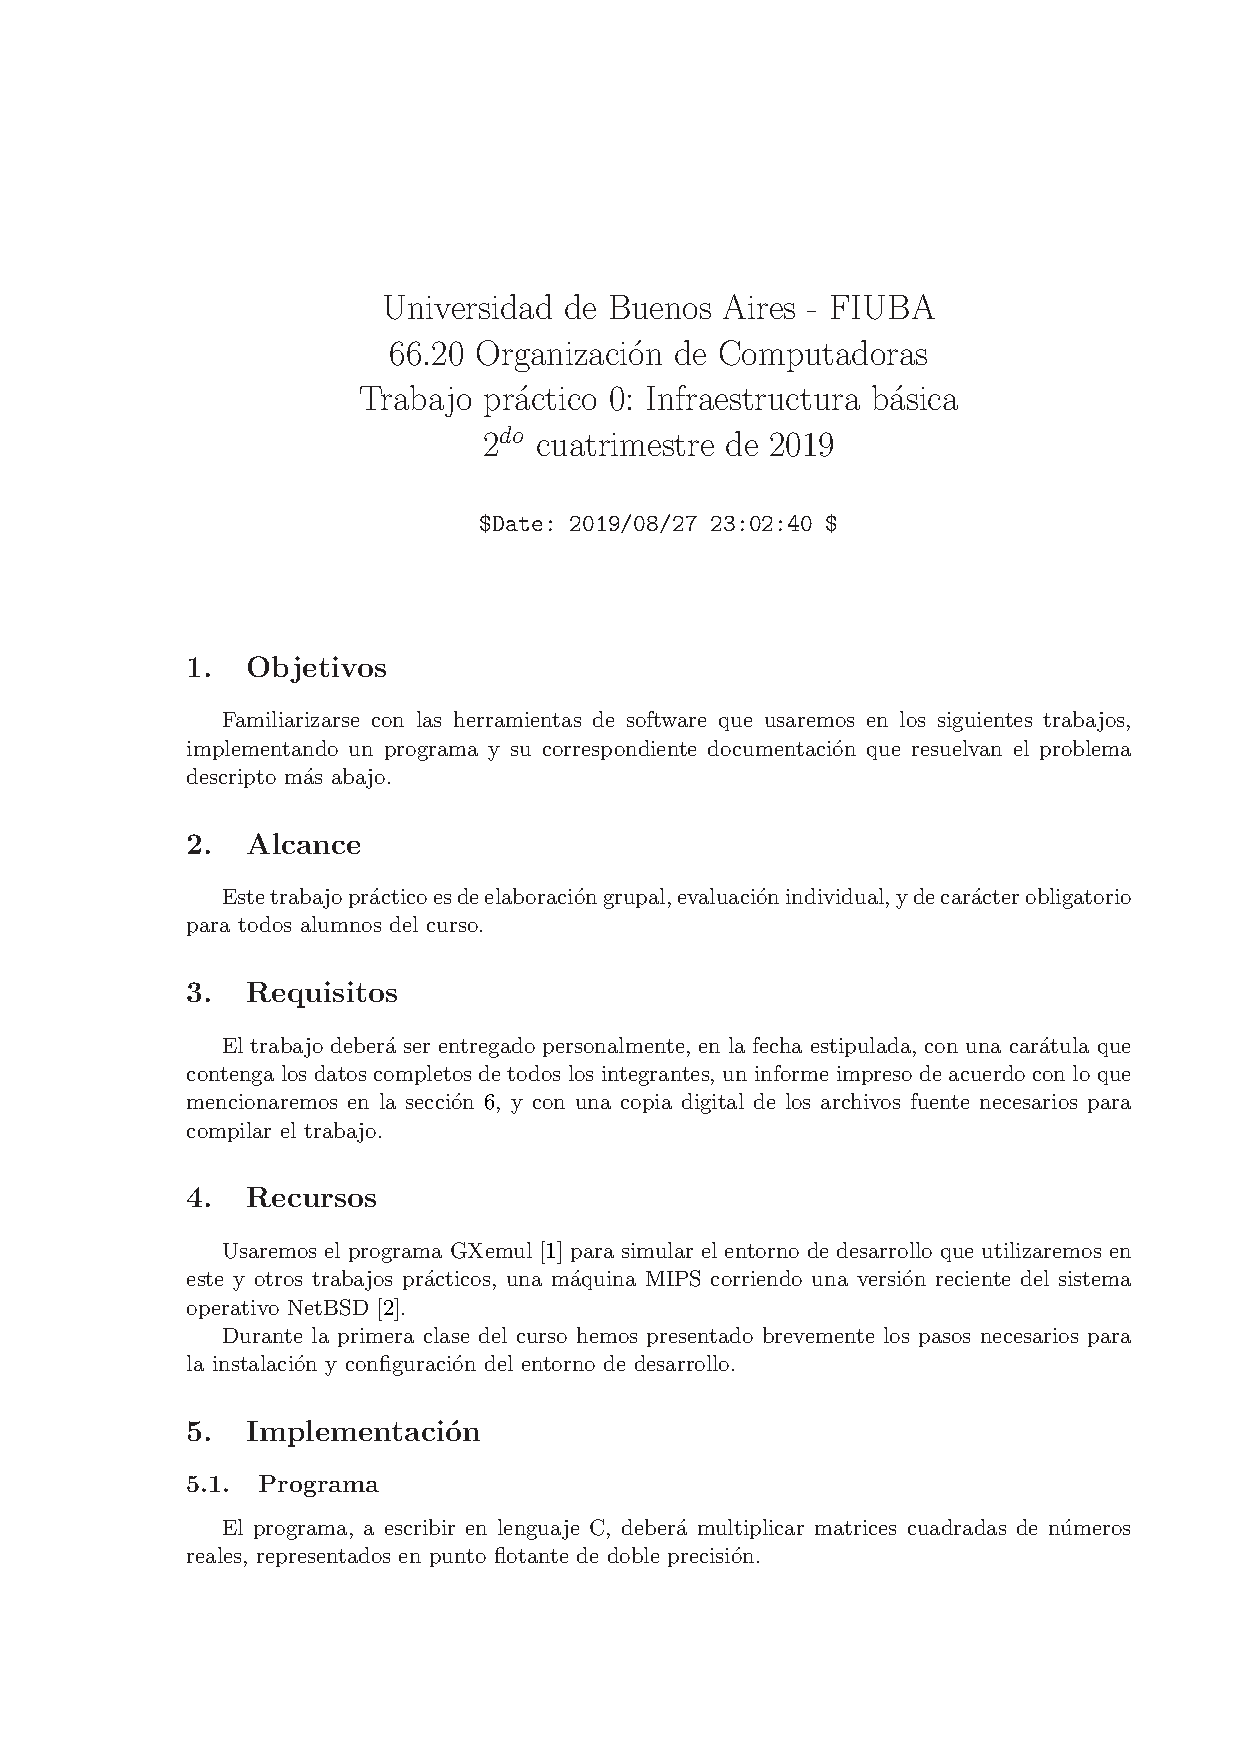
\includepdf[
    trim=20mm 30mm 10mm 25mm, clip,
    pages=1,
    frame,
    scale=.65,
    pagecommand=\section{Enunciado}
 ]{tp0-2019-2q.pdf}
\includepdf[
    trim=20mm 30mm 10mm 25mm, clip,
    pages=2-,
    frame,
    scale=.65,
    pagecommand={}
 ]{tp0-2019-2q.pdf}

\section{Solución}

\subsection{Diseño}

La solución propuesta para este trabajo comprende una serie de funciones que pueden ser clasificadas según una determinada división de responsabilidades:

\begin{itemize}
	\item \textbf{Procesamiento:} Comprende las funciones dedicadas a lectura y procesamiento de datos para obtener las matrices a multiplicar.
  \item \textbf{Buffering:} El procesamiento requiere la utilización de un buffer dinámico que almacene los valores numéricos de punto flotante de doble precisión, que primero 
  son almacenados como un array de \lstinline{char}, y luego convertidos al tipo \lstinline{double}.
  \item \textbf{Implementación de matrices:} Esta parte comprende la interfaz definida por el enunciado para la creación, impresión, multiplicación y destrucción de matrices.
  \item \textbf{Presentación:} Refiere al código generado para imprimir menús y mensajes de error.
\end{itemize}

\subsubsection{Buffering}

Este fragmento de la solución contiene las funciones \lstinline{initBuffer} y \lstinline{push}. La primer función inicializa el buffer. 
La segunda, agrega caracteres a un buffer ingresado como arugmento, manejando dinámicamente la memoria alocada por el buffer on demand.

\subsubsection{Procesamiento}

Esta parte cuenta con las siguientes funciones: 

\begin{itemize}
  \item \lstinline{getValue:} Esta función escribe sobre un puntero pasado como argumento el valor de punto flotante obtenido, correspondiente a una 'palabra' leida por \lstinline{stdin}. 
  Esta misma función se utiliza para leer el primer valor entero que indica el tamaño de la matriz cuadrada. Por ello luego se castea el valor obtenido a un entero.
	\item \lstinline{tryOpenFile:} Encargada de abrir los streams de input y output, según los
  argumentos con los que se invoque la función. Por default esta función utiliza \lstinline{stdin} 
  y \lstinline{stdout} como input y output stream respectivamente.
\end{itemize}


\subsubsection{\lstinline{Unix2dos}}

El cuerpo principal del programa \lstinline{unix2dos} consiste en los siguientes pasos.

\begin{enumerate}
	\item Obtener los nombres de los archivos de entrada y salida a partir de los argumentos de la
	ejecución, utilizando la función \lstinline{getFileName}.
	\item Abrir los archivos de input y output especificados, o en su defecto, \lstinline{stdin} y \lstinline{stdout},
	invocando a la función \lstinline{tryOpenFile}.
	\item Recorrer el stream de entrada con un puntero escribiendo cada caracter en el output stream
  correspondiente, a excepción de los caracteres \lstinline{`\n'}, los cuales serían escritos como
  \lstinline{`\r\n'}.
\end{enumerate}

El siguiente es el código correspondiente a \lstinline{unix2dos.c}.

\subsubsection{\lstinline{Dos2unix}}

\lstinline{Dos2unix} tiene escencialmente el mismo comportamiento que \lstinline{unix2dos},
excepto que al recorrer el stream de entrada, son las suceciones de caracteres \lstinline{`\r\n'}
las que son escritas como el caracter \lstinline{`\n'}.


\lstset{
  language=bash,
  basicstyle=\small\ttfamily
}

\subsection{Compilación del programa}
Para compilar el programa sencillamente tenemos utilizar su makefile desde el directorio donde se descomprimió el entregable:
\begin{lstlisting}
$ gmake all
cc -I. -c common.c -o obj/common.o -std=c99 -Wall -Werror -pedantic -pedantic-errors
cc -I. -c dos2unix.c -o obj/dos2unix.o -std=c99 -Wall -Werror -pedantic -pedantic-errors
cc -I. -c unix2dos.c -o obj/unix2dos.o -std=c99 -Wall -Werror -pedantic -pedantic-errors
cc obj/common.o obj/unix2dos.o -o unix2dos
cc obj/common.o obj/dos2unix.o -o dos2unix
	
\end{lstlisting}

\section{Casos de prueba}

\subsection{Casos elegidos}

Los casos de prueba elegidos se distribuyen en 3 grupos: DOS, UNIX y mixed. \\
DOS y UNIX contienen los mismos casos, excepto que en DOS los casos tienen \textit{line endings}
con \lstinline{`\r\n'} y en UNIX con \lstinline{`\n'}.

En mixed se agrupan los casos neutros, que corresponden a pruebas con archivos vacíos o con ocurrencias
de ambos tipos de \textit{line endings}.

\subsubsection{Simple.txt}

Simple.txt es la prueba básica para evaluar el correcto funcionamiento de los programas.
Su contenido es simplemente el siguiente.

\begin{lstlisting}
  One line
  two lines
  three lines
\end{lstlisting}

Por ejemplo, la ejecución del archivo \lstinline{simple.txt} de la carpeta UNIX con el programa
\lstinline{unix2dos} es la siguiente:

\begin{lstlisting}
$ ./unix2dos -i casos_prueba/UNIX/simple.txt | od -t c
0000000   O   n   e       l   i   n   e  \r  \n   t   w   o       l   i
0000020   n   e   s  \r  \n   t   h   r   e   e       l   i   n   e   s
0000040  \r  \n
0000042
\end{lstlisting}
Ejecución con valgrind:
\begin{lstlisting}
$ valgrind --leak-check=yes ./unix2dos -i casos_prueba/UNIX/simple.txt -o nuevoarchivo.txt

==7662== Memcheck, a memory error detector
==7662== Copyright (C) 2002-2017, and GNU GPL'd, by Julian Seward et al.
==7662== Using Valgrind-3.13.0 and LibVEX; rerun with -h for copyright info
==7662== Command: ./unix2dos -i casos_prueba/UNIX/simple.txt -o nuevoarchivo.txt
==7662== 
==7662== 
==7662== HEAP SUMMARY:
==7662==     in use at exit: 0 bytes in 0 blocks
==7662==   total heap usage: 4 allocs, 4 frees, 9,296 bytes allocated
==7662== 
==7662== All heap blocks were freed -- no leaks are possible
==7662== 
==7662== For counts of detected and suppressed errors, rerun with: -v
==7662== ERROR SUMMARY: 0 errors from 0 contexts (suppressed: 0 from 0)
\end{lstlisting}

Puede verse así que en la ejecución no se pierde memoria, y se llega al resultado esperado.
En este caso los cortes de línea se reemplazan por \lstinline{`\r\n'}.

\subsubsection{Complex.txt y complex\_long.txt}

Los archivos complex y complex\_long.txt prueban nuestros programas ante archivos con caracteres
extraños. Complex\_long.txt se caracteriza por tener líneas muy largas.

La siguiente es la ejecución de \lstinline{dos2unix} con el archivo DOS/complex.txt. 

\begin{lstlisting}
$ ./dos2unix -i casos_prueba/DOS/complex.txt | od -t c
  0000000 304 252 302 264 304 207   k 302 210 302 222 303 270   K   X   y
  0000020 304 261 304 231 302 212   U 304 203 302 250   M 302 256   K 303
  0000040 250 303 233     302 254 303 244 302 212 304 237   u 303 250   M
  0000060 303 266 303 220   E   b 303 225 302 270 304 206 302 254 302 201
  0000100 303 204   R 303 224 304 260   C   b   | 302 245 304 241 304 207
  0000120   L 304 257 303 236 303 225   s   p 304 245 304 260   A   o 303
  0000140 224   W   {   o 303 202 303 222 304 267 304 241 302 200   G 303
  0000160 235   w 302 256   p   k   L   i   c 304 231 302 221   p   s 303
  0000200 272 303 232 304 217 304 241 304 202   N 302 252 303 256 302 202
  0000220   O 303 253   J   d 302 241   _   R 303 226 303 202   a 303 236
  0000240 304 255 303 257 304 272   M 304 233 304 252 304 264 304 220   \
  0000260 302 242 304 221 303 261 302 267   j 302 222 304 242 302 213 304
  0000300 212 303 263 302 212   O   ^   O 303 251 302 213 304 213   h 302
  0000320 270 304 236   Y 302 216 304 267 302 214 304 256 304 273   [ 302
  0000340 246 303 224 302 234   { 303 233 304 255   d   i   a   p 302 272
  0000360 302 252 304 223   l 304 266   Z 304 205 302 225 303 220 302 222
  0000400 303 267 302 211 304 211   B 304 206 302 220 302 231   h   G 304
  0000420 272   p   D   k 303 221 302 245 302 233   T 304 215 303 204   g
  0000440 303 241 302 270 302 247   N 304 273   } 302 232   k 303 201 177
  0000460   Y 304 270   \ 304 256 303 220 304 275 304 257 304 215 304 250
  0000500 304 241   m 304 230 303 243   O 302 227 304 264 302 276 302 221
  0000520 302 254 303 204   Y 302 224 303 212 302 264   q 304 222 304 273
  0000540   E   L 302 273 303 231   T   G 304 203 304 213   W 304 255   t
  0000560   y 304 214   e 304 255 303 221 303 274 304 220 302 212 303 203
  0000600 304 233   | 302 245 304 200   p 304 231     302 235 302 201   H
  0000620 304 260 303 267 304 200   P 304 257 303 233 304 221 304 200   ]
  0000640   n  \n   ^ 303 235 303 272 302 206 304 211 302 244   F 304 236
  0000660 303 267 304 200 302 234 304 271 302 233 302 246   } 304 255 303
  0000700 235   Y   N 302 226 302 206 304 244 177 302 270 303 250 302 264
  0000720 303 254 302 227 303 230   i 304 246 303 257 303 265 304 207 304
  0000740 264 304 224 304 217 303 212 303 247   c 304 223   h 303 211 303
  0000760 201 302 230 303 272 303 211 303 257   a 302 211   Y 304 220 303
  0001000 241 302 265   B 302 221 303 233 304 203 303 266 302 241   l 304
  0001020 263 302 200 302 271 302 273 303 217 302 225 304 200   j 302 203
  0001040   X   Y   D 303 270 304 217 302 252 302 230 303 257 303 244   ^
  0001060 302 206 304 265 304 200   F 304 244 303 242   j 304 237   ` 304
  0001100 252       P 302 247 302 225 304 214 302 252 303 213   w 304 262
  0001120   h 304 221 303 204 302 253 304 227   i 303 247 304 235   W 304
  0001140 221 302 255 302 250 302 226 304 226 302 271   O 303 246 302 251
  0001160 302 251 302 275 303 232 303 235 302 272 304 234 304 265 302 270
  0001200 302 254 302 212 304 225 304 204 302 210 303 212 303 207 302 251
  0001220   s 302 242   c 302 224 304 265   ` 302 242   p 302 277   Z 302
  0001240 273 304 224 304 233 303 266 303 257 304 273 303 261 303 257 303
  0001260 261 303 263   _ 304 244 302 222 302 244 302 254 302 253 303 252
  0001300   E 304 273   d 303 247 302 231   y   e     304 261 303 243 302
  0001320 211   X   ]   n 304 266  \n   H 302 261   k 302 265 302 234   a
  0001340 302 261 302 230   c   M 302 204   Q   h 302 246 303 201 302 256
  0001360   k 304 204 302 227 302 241 303 265 304 272   | 304 252 302 214
  0001400 303 227 304 261 303 263 303 274   R   n 303 206 302 277   ] 304
  0001420 233 303 241   V 304 253 303 207 303 210   B 303 223 303 252 302
  0001440 265 303 240   L 304 225 304 274 304 203 303 261 303 244 303 274
  0001460   j 302 205 303 262 304 222 304 243   o   q 304 201 304 221 304
  0001500 223 302 235 302 235 304 202 302 262 304 251 304 202 302 211 303
  0001520 274   ` 304 236 304 264 303 277   l 303 205 303 232 302 215   L
  0001540   m 303 251   D 302 220 303 215 304 244 303 217 303 214   A 303
  0001560 276 302 265 303 245 303 207   p 302 256 303 214 302 264 303 223
  0001600 302 245 302 225   g 302 272 304 210   k 304 271 303 250   s 304
  0001620 230 303 261 302 277 303 251 304 263 303 256 304 207 304 267   D
  0001640 304 250   B 303 224 302 243 302 276 304 235 304 200   ^ 302 223
  0001660 302 231 304 252   E 302 201 304 223 303 273 304 255 302 244 303
  0001700 254 302 230 303 256 304 221 304 204 302 202 304 222   n   j 302
  0001720 262   C 303 223 302 271 304 213 304 202 304 213 303 201 303 220
  0001740 304 243 302 201 304 266 304 250   c 302 243 303 245 303 261 304
  0001760 221 303 202   j 302 277 303 277 303 245 302 211 302 276 303 232
  0002000   C   ] 303 275 304 260 304 253 303 251 304 274 302 200 304 236
  0002020 303 231 304 213 302 215 303 212   S 303 266   }   A 302 247 303
  0002040 237   a 303 217 303 254 303 213   ] 302 274 304 227   D 302 200
  0002060 302 230 304 254 304 213 302 246   { 302 212 303 245 302 250 303
  0002100 267 303 202 304 216 303 252   o   ^   r 302 224 302 275   j 303
  0002120 242 304 260 303 220   Q 302 252   J 302 244 302 241   R 303 204
  0002140   V 303 263 304 233 303 223 304 244 303 260 304 220 302 255   F
  0002160 304 270 302 262 303 226 303 230 304 273 303 215 303 271 304 261
  0002200 302 247 303 203 303 222 302 203 303 231 303 265 302 276 303 214
  0002220 303 240   J 302 263 302 274 304 266 303 236 304 250 304 260 303
  0002240 235 302 261   j 302 207   O   w 302 251 302 204 303 231 302 220
  0002260 302 235   i 304 234 303 271   |  \n
  0002271  
\end{lstlisting}
En esta ejecución se muestra la varidedad de caracteres utilizados y el resultado 
de reemplazar los cortes de línea por caracteres \lstinline{`\n'}. Los caracteres extraños
no afectan la normal ejecución del programa.
\subsubsection{Big.txt}
El archivo Big.txt corresponde a un documento de texto normal, escrito mayormente en inglés, pero sumamente
grande (pesa 6.6Mb).
La ejecución con valgrind de este archivo muestra que la memoria alocada por el programa es la misma
indistintamente del tamaño del archivo, dado que se utiliza sólamente un puntero para recorrerlo, tanto en
\lstinline{unix2dos} como en \lstinline{dos2unix}.
Ejecución con valgrind:
\begin{lstlisting}
$ valgrind --leak-check=yes ./unix2dos -i casos_prueba/UNIX/big.txt
  ==5509== Memcheck, a memory error detector
  ==5509== Copyright (C) 2002-2017, and GNU GPL'd, by Julian Seward et al.
  ==5509== Using Valgrind-3.13.0 and LibVEX; rerun with -h for copyright info
  ==5509== Command: ./unix2dos -i casos_prueba/UNIX/big.txt -o nuevoarchivo.txt
  ==5509== 
  ==5509== 
  ==5509== HEAP SUMMARY:
  ==5509==     in use at exit: 0 bytes in 0 blocks
  ==5509==   total heap usage: 4 allocs, 4 frees, 9,296 bytes allocated
  ==5509== 
  ==5509== All heap blocks were freed -- no leaks are possible
  ==5509== 
  ==5509== For counts of detected and suppressed errors, rerun with: -v
  ==5509== ERROR SUMMARY: 0 errors from 0 contexts (suppressed: 0 from 0)  
\end{lstlisting}
\subsubsection{Empty.txt y oneliner.txt}
Estos archivos constituyen básicamente un archivo vacío y un archivo de una línea respectivamente.
Son casos utilizados para verificar la normal ejecución del programa en los casos borde de un archivo
vacío o con tan sólo una línea.
La siguiente es por ejemplo la ejecución de \lstinline{dos2unix} con oneliner.txt:
\begin{lstlisting}
  $ ./dos2unix -i casos_prueba/mixed/oneliner.txt | od -t c
  
  0000000   h   e   l   l   o       t   h   i   s       i   s       a    
  0000020   l   i   n   e
  0000024    
\end{lstlisting}
La ejecución resulta normal y naturalmente no debe reemplazarse ningún caracter.
\subsubsection{Mixed.txt}
Mixed.txt es un archivo que contiene ambos tipos de fin de línea.
A continuación se puede ver el contenido del archivo:
\begin{lstlisting}
  $ cat casos_prueba/mixed/mixed.txt | od -t c
  0000000  \r  \n  \n  \r  \n  \r  \n  \n  \n  \r  \r  \n  \n  \n  \r  \r
  0000020  \r  \r  \n  \r  \n
  0000025
\end{lstlisting}
La siguiente es la ejecución de \lstinline{dos2unix} con este archivo:
\begin{lstlisting}
  $ ./dos2unix -i casos_prueba/mixed/mixed.txt | od -t c
  0000000  \n  \n  \n  \n  \n  \n  \r  \n  \n  \n  \r  \r  \r  \n  \n
  0000017  
\end{lstlisting}
Como puede verse las sucesiones \lstinline{`\r\n'} son reemplazadas por \lstinline{`\n'},
mientras que algunos caracteres \lstinline{`\r'} sobrantes son ignorados al no coincidir
con la secuencia que debe reemplazarse por fines de línea estilo UNIX.


\section{Código MIPS}

\subsection{Código assembly generado para \textit{common}}

\lstset{ %
  language=[mips]Assembler,
  backgroundcolor=\color{white},
  showspaces=false,
  showstringspaces=false,
  showtabs=false,
  frame=single,
  rulecolor=\color{black},
  tabsize=4,
  captionpos=b
  breaklines=true,
  breakatwhitespace=false,
  title=\lstname,
  keywordstyle=\color{blue},
  commentstyle=\color{dkgreen},
  stringstyle=\color{mauve},
  escapeinside={\%*}{*)},
  morekeywords={*,...}
}

\subsection{Código assembly generado para \textit{unix2dos}}

\lstset{ %
  language=[mips]Assembler,
  backgroundcolor=\color{white},
  showspaces=false,
  showstringspaces=false,
  showtabs=false,
  frame=single,
  rulecolor=\color{black},
  tabsize=4,
  captionpos=b
  breaklines=true,
  breakatwhitespace=false,
  title=\lstname,
  keywordstyle=\color{blue},
  commentstyle=\color{dkgreen},
  stringstyle=\color{mauve},
  escapeinside={\%*}{*)},
  morekeywords={*,...}
}

\subsection{Código assembly generado para \textit{dos2unix}}

\lstset{
  language=[mips]Assembler,
  backgroundcolor=\color{white},
  showspaces=false,
  showstringspaces=false,
  showtabs=false,
  frame=single,
  rulecolor=\color{black},
  tabsize=4,
  captionpos=b
  breaklines=true,
  breakatwhitespace=false,
  title=\lstname,
  keywordstyle=\color{blue},
  commentstyle=\color{dkgreen},
  stringstyle=\color{mauve},
  escapeinside={\%*}{*)},
  morekeywords={*,...}
}

\section{Conclusiones}

A modo de conclusión podemos decir que en este trabajo práctico pudimos configurar y familiarizarnos con el entorno de trabajo de la materia, que emula una computadora con procesador MIPS. 
También pudimos observar algunas de las diferencias entre programar para un sistema operativo linux y para el netBSD que corre emulado. Además adquirimos conocimiento respecto a otras herramientas útiles como ssh, scp, diff y od entre otras.


\end{document}
